\documentclass[aspectratio=169,10pt]{beamer}

% fallback search path for ../theme/ when TEXINPUTS is not set (e.g. texmaker
% quick build); the makefile's TEXINPUTS takes precedence, so no conflict
\makeatletter
\providecommand*{\input@path}{}
\edef\input@path{\input@path{../theme/}{../theme/moloch/}}
\makeatother
\usepackage{icl26}

\title{Variational inequalities and their finite element solutions}
\subtitle{A genuine introduction}
\author{Ed Bueler}
\institute{University of Alaska Fairbanks}
\date{Imperial College London \, 2026}

\newcommand{\cK}{{\mathcal{K}}}  % outer braces: safe in P_\cK under unicode-math
\newcommand{\ip}[2]{\left\langle #1, #2 \right\rangle}

\begin{document}

\begin{frame}
  \titlepage
\end{frame}

\begin{frame}{outline}
  \tableofcontents
\end{frame}


\section[finite-dimensional examples]{finite-dimensional examples \hfill {\small \texorpdfstring{$\leftarrow$}{←} \emph{geometry of VIs}}}

\begin{frame}{a calculus I problem}

\begin{itemize}
\item minimize smooth $f(x)$ over a closed interval $[a,b]$?
\item what we tell our students: \quad $f'(x)=0$, but test the end-points

\medskip
  \centering
  \only<1>{\begin{tikzpicture}[x=0.95cm, y=1.0cm,
                    fn/.style={icBlue, very thick, domain=0:6, samples=120}]
  \useasboundingbox (-3.1,-1.1) rectangle (9.1,1.9);  % same size as calcIcases.tex
  \draw[icNavy] (-0.3,0) -- (6.3,0);
  \draw[icNavy] (0,0.08) -- (0,-0.08) node[below] {$a$};
  \draw[icNavy] (6,0.08) -- (6,-0.08) node[below] {$b$};
  \draw[fn] plot (\x, {0.9 + 0.35*sin(deg(2.1*\x+0.5)) + 0.25*sin(deg(4.3*\x))
                       + 0.04*(\x-3.5)^2});
  \node[icBlue] at (6.25,1.6) {$f$};
  % global minimum
  \fill (2.444,0.512) circle (1.8pt);
  \draw[icNavy] (2.444,0.08) -- (2.444,-0.08) node[below] {$u$};
\end{tikzpicture}
}%
  \only<2->{\begin{tikzpicture}[x=0.95cm, y=1.0cm,
                    fn/.style={icBlue, very thick, domain=0:3, samples=40},
                    tan/.style={icAccent, thick, dashed}]
  \useasboundingbox (-0.2,-1.1) rectangle (12,1.9);  % shared with calcIgeneric.tex
  \foreach \xo/\la/\lb/\cond in {0/a/b/{$f'(u)=0$},
                              4.4/a=u/b/{$f'(u)\ge 0$},
                              8.8/a/u=b/{$f'(u)\le 0$}} {
    \begin{scope}[xshift=\xo cm]
      \draw[icNavy] (-0.2,0) -- (3.2,0);
      \draw[icNavy] (0,0.08) -- (0,-0.08) node[below] {$\la$};
      \draw[icNavy] (3,0.08) -- (3,-0.08) node[below] {$\lb$};
      \node at (1.5,-0.85) {\cond};
    \end{scope}
  }
  % interior minimum
  \draw[fn] plot (\x, {0.5 + 0.4*(\x-1.8)^2});
  \draw[tan] (1.2,0.5) -- (2.4,0.5);
  \fill (1.8,0.5) circle (1.8pt);
  \draw[icNavy] (1.8,0.08) -- (1.8,-0.08) node[below] {$u$};
  % minimum at left endpoint
  \begin{scope}[xshift=4.4cm]
    \draw[fn] plot (\x, {0.5 + 0.45*\x - 0.06*\x^2});
    \draw[tan] (0,0.5) -- (1.2,1.04);
    \fill (0,0.5) circle (1.8pt);
  \end{scope}
  % minimum at right endpoint
  \begin{scope}[xshift=8.8cm]
    \draw[fn] plot (\x, {0.5 + 0.25*(3-\x) + 0.08*(3-\x)^2});
    \draw[tan] (3,0.5) -- (1.8,0.8);
    \fill (3,0.5) circle (1.8pt);
  \end{scope}
\end{tikzpicture}
}

\raggedright
\item<2-> 3 cases arise for a minimizer $u$
\item<3-> all cases are captured by this \alert{variational inequality} (VI):
  $$\alert{f'(u)\,(x-u) \ge 0} \qquad \text{for all } x\in[a,b]$$

\quad \grey{\small as you travel from $u$ into $[a,b]$, $f$ \strikeThrough{slopes upward} does not slope downward}
\end{itemize}
\end{frame}


\begin{frame}{projection onto a closed, convex set}

\begin{itemize}
\item suppose $H$ is a Hilbert space \grey{(e.g.~$\mathbb{R}^n$)}
\item let $K\subset H$ be a nonempty, closed, and convex subset

\begin{definition}
for $x\in H$, define the \emph{projection} of $x$ onto $K$:
  $$u = \Pi_K x = \operatorname*{argmin}_{y\in K}\, \|y-x\| \hspace{50mm}$$
\grey{\small (a parallelogram and completeness argument}

\noindent \grey{\small shows $u$ exists and is unique)}

\vspace{-25mm}
\hfill \begin{tikzpicture}[scale=0.85, rotate=-15]
  \fill[icBlue!12] (1,0.5) -- (3.5,0.2) -- (4,2) -- (2.2,3) -- (1,2.5) -- cycle;
  \draw[icBlue, thick] (1,0.5) -- (3.5,0.2) -- (4,2) -- (2.2,3) -- (1,2.5) -- cycle;
  \node[icBlue] at (3.2,1.2) {$K$};
  \fill (-0.4,1.6) circle (1.8pt) node[left] {$x$};
  \draw[-{Stealth}, icNavy, thick] (-0.4,1.6) -- (1,1.6);
  \fill (1,1.6) circle (1.8pt) node[below right] {$y$};
  \uncover<2->{
    \draw[icGrey, dashed] (1,1.6) -- (2,1.6);
    \draw[-{Stealth}, icAccent, thick] (1,1.6) -- (2.6,2.4);
    \fill (2.6,2.4) circle (1.8pt) node[above right] {$\eta$};
  }
\end{tikzpicture}


\medskip
\end{definition}

\pause
\item but how do we characterize $u=\Pi_K x$ by its geometrical properties?
\pause
\item $u=\Pi_K x\in K \qquad \iff \alert{\ip{u-x}{y-u}\ge 0} \quad \text{for all } y\in K$

\quad \grey{\small angle between $u-x$ and $y-u$ is at most $90^\circ$ (not obtuse)}
\end{itemize}
\end{frame}


\begin{frame}{minimize $f$ over a convex set $K\subset\mathbb{R}^n$}
\begin{theorem}
\begin{minipage}{0.6\linewidth}
let $K\subset\mathbb{R}^n$ be convex and $f\in C^1$; if $u\in K$ minimizes $f$ over $K$ then
  $$\nabla f(u)\cdot(v-u)\ge 0 \qquad\text{for all } v\in K$$
\end{minipage}
\hfill
\begin{minipage}{0.36\linewidth}
  \centering
  \scalebox{0.75}{\begin{tikzpicture}[scale=0.85, rotate=20]
  \fill[icBlue!12] (0,0.3) -- (2,0.6) -- (2,2.6) -- (0.6,3) -- (-0.4,1.6) -- cycle;
  \draw[icBlue, thick] (0,0.3) -- (2,0.6) -- (2,2.6) -- (0.6,3) -- (-0.4,1.6) -- cycle;
  \node[icBlue] at (0.5,2.2) {$K$};
  \foreach \s in {0.5,1,1.5}
    \draw[icGrey] (3.4,1.7) ellipse ({1.4*\s} and {0.8*\s});
  \fill[icGrey] (3.4,1.7) circle (1.5pt);
  \draw[-{Stealth}, icAccent, thick] (2,1.7) -- (2.9,1.7)
    node[below, pos=0.75] {\small $-\nabla f$};
  \coordinate (v) at (0.7,0.9);
  \draw[-{Stealth}, icNavy] (2,1.7) -- (v);
  \fill (v) circle (1.5pt) node[below left] {$v$};
  \fill (2,1.7) circle (1.8pt) node[above left] {$u$};
\end{tikzpicture}
}

  {\small level sets of $f$}
\end{minipage}
\end{theorem}

\pause
\emph{proof:}\, for $v\in K$, $u+t(v-u)\in K$ for $0\le t\le 1$, so
$t=0$ minimizes $g(t)=f(u+t(v-u))$ on $[0,1]$; by the calculus I problem,
$0\le g'(0)=\nabla f(u)\cdot(v-u)$ \qed

\pause
\begin{itemize}
\item if $f$ is convex then the VI is also \emph{sufficient}
\item exists if $K$ compact \grey{(or closed, with $f$ coercive)}
\item unique if $f$ strictly convex
\item FIXME example; $f(u) = \tfrac{1}{2} \|u-x\|^2$ on previous
\end{itemize}
\end{frame}


\begin{frame}{nonlinear equations $F(x)=0$}
  given continuous $F:\mathbb{R}^n\to\mathbb{R}^n$, find $x$ so that $F(x)=0$
  \begin{itemize}
    \item there is little positive to say in general: no existence
          \grey{(e.g.~$F(x)=e^x$)}, no uniqueness
  \end{itemize}

  \pause
  \medskip
  change the problem minimally: seek $x$ in a compact, convex $K\subset\mathbb{R}^n$
  \begin{theorem}[Hartman \& Stampacchia, 1966]
    if $K\subset\mathbb{R}^n$ is nonempty, compact, and convex, and $F$ is continuous,
    then there exists $x\in K$ so that
    $$
      F(x)\cdot(y-x)\ge 0 \qquad\text{for all } y\in K
    $$
  \end{theorem}
  \pause
  \begin{itemize}
    \item if $x$ is in the interior of $K$ then $F(x)=0$ \grey{(take $y=x\pm\epsilon e_i$)}
    \item for $K=\mathbb{R}^n$ the VI \emph{is} $F(x)=0$ \grey{(but $\mathbb{R}^n$ is not compact)}
    \item example: $F(x)=e^x$ on $K=[a,b]$ has solution $x=a$
  \end{itemize}
\end{frame}

\begin{frame}{proof: a fixed point of a projected map}
  \begin{columns}[T]
    \begin{column}{0.58\textwidth}
      the map $x'\mapsto P_K\big(x'-F(x')\big)$ is continuous from $K$ to $K$, so by
      Brouwer it has a fixed point:
      $$
        x = P_K z, \qquad z = x - F(x).
      $$
      \pause
      by the projection theorem, for all $y\in K$,
      $$
        0 \le \ip{P_K z - z}{y - P_K z} = F(x)\cdot(y-x). \qquad\qed
      $$
      \pause
      \begin{itemize}
        \item converse: VI solutions are fixed points of
              $x\mapsto P_K(x-\rho F(x))$ for any $\rho>0$
        \item \alert{projection} is the basic geometric operation for VIs
      \end{itemize}
    \end{column}
    \begin{column}{0.4\textwidth}
      \centering
      \begin{tikzpicture}[scale=0.85]
  \fill[icBlue!12] (1,0.4) -- (3.4,0.6) -- (3.8,2.4) -- (2.4,3.2) -- (1,2.7) -- cycle;
  \draw[icBlue, thick] (1,0.4) -- (3.4,0.6) -- (3.8,2.4) -- (2.4,3.2) -- (1,2.7) -- cycle;
  \node[icBlue] at (3,1.3) {$K$};
  \draw[-{Stealth}, icAccent, thick] (1,1.5) -- (-0.4,1.5)
    node[above, pos=0.5] {\small $-F(x)$};
  \fill (-0.4,1.5) circle (1.8pt) node[left] {$z$};
  \fill (1,1.5) circle (1.8pt) node[below right] {$x$};
  \draw[-{Stealth}, icNavy] (1,1.5) -- (2.7,2.5);
  \fill (2.7,2.5) circle (1.5pt) node[above right] {$y$};
\end{tikzpicture}

    \end{column}
  \end{columns}
\end{frame}

\begin{frame}{what is a variational inequality?}
  \begin{definition}
  given a closed, convex $K\subset\mathcal{H}$ and $F:K\to\mathcal{H}'$, find $u\in K$ so that
  $$
    \ip{F(u)}{v-u} \ge 0 \qquad \text{for all } v\in K
  $$
  \end{definition}
  {\centering\small
    \begin{tabular}{lll}
      \toprule
      problem                     & $K$                      & $F(u)$ \\
      \midrule
      calculus I                  & $[a,b]$                  & $f'(u)$ \\
      minimize $f$ over $K$       & convex                   & $\nabla f(u)$ \\
      projection of $x$ onto $K$  & closed, convex           & $u-x$ \\
      nonlinear equations         & compact, convex          & $F(u)$ \\
      \midrule
      $F(u)=0$                    & $\mathcal{H}$            & $F(u)$ \\
      \bottomrule
    \end{tabular}
  \par}
  \pause
  \begin{itemize}
    \item VIs generalize equations, and not every VI is a minimization
    \item \emph{next:} $K\subset$ a function space, $F$ from a PDE
  \end{itemize}
\end{frame}


\AtBeginSection[]
{
  \begin{frame}{outline}
  \tableofcontents[currentsection]
  \end{frame}
}


\section[infinite-dimensional examples]{infinite-dimensional examples \hfill {\small \texorpdfstring{$\leftarrow$}{←} \emph{some applications of VIs}}}

\begin{frame}{the classical obstacle problem}
  an elastic membrane over $\Omega\subset\mathbb{R}^d$, with small vertical displacement $u$,
  fixed $u=g$ on $\partial\Omega$, under force $f$, and constrained to lie above an obstacle $\psi$:
  $$
    u-\psi\ge 0, \qquad -\nabla^2 u - f \ge 0, \qquad (u-\psi)(-\nabla^2 u - f) = 0
    \qquad \text{a.e.~in } \Omega
  $$
  \vspace{-3mm}
  \begin{columns}[T]
    \begin{column}{0.45\textwidth}
      \begin{itemize}
        \item \emph{inactive set} $E_u=\{u>\psi\}$: \\ Poisson $-\nabla^2 u=f$ holds
        \item \emph{active} or \emph{contact set} \\ $C_u=\Omega\setminus E_u$: $u=\psi$
        \item \emph{free boundary} $\Gamma_u=\Omega\cap\partial E_u$
      \end{itemize}
    \end{column}
    \begin{column}{0.53\textwidth}
      \centering
      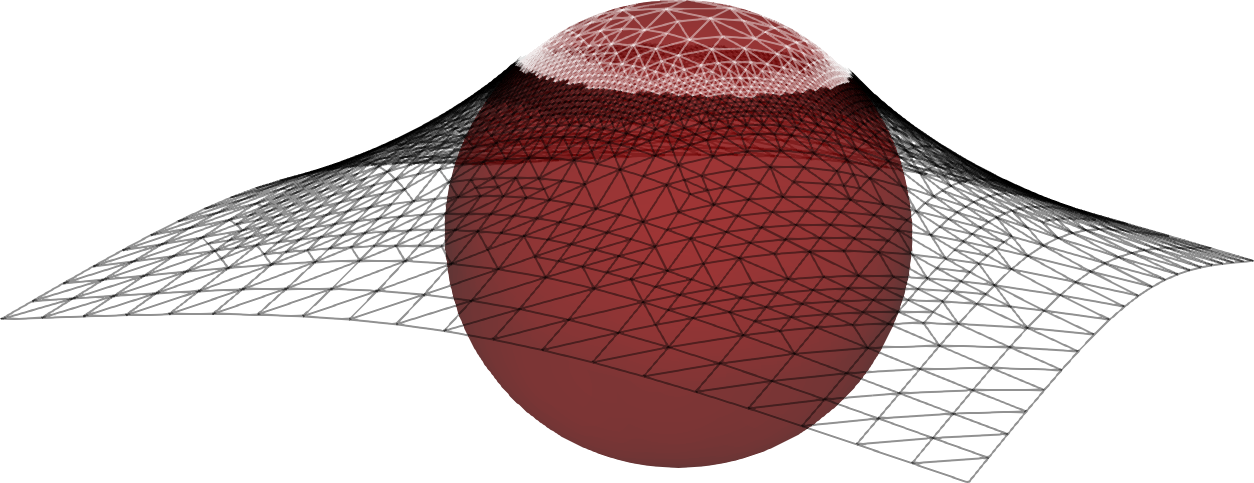
\includegraphics[width=\textwidth]{figs/viamr-obstacle.png}

      {\scriptsize \grey{hemisphere obstacle; contact set is a disc \quad
      (Fochesatto \& Bueler, VIAMR)}}
    \end{column}
  \end{columns}
\end{frame}

\begin{frame}{obstacle problem: weak form}
  let $\cK = \{v\in H^1(\Omega) : v\ge\psi \text{ and } v|_{\partial\Omega}=g\}$, a closed, convex set
  but \alert{not} a subspace; find $u\in\cK$ so that
  $$
    \int_\Omega \nabla u\cdot\nabla(v-u) \ge \int_\Omega f\,(v-u)
    \qquad \text{for all } v\in\cK
  $$
  \begin{itemize}
    \item equivalent to minimizing $J(v)=\int_\Omega \tfrac12|\nabla v|^2 - fv$ over $\cK$
    \item integrate by parts: $\ip{\sigma}{v-u}\ge 0$ for the residual $\sigma=-\nabla^2u-f$
    \begin{itemize}
      \item[$\circ$] if $u$ is in the interior of $\cK$ then $\sigma=0$: the VI generalizes Poisson
    \end{itemize}
    \item both $u=\psi$ \emph{and} $\partial(u-\psi)/\partial n=0$ hold along $\Gamma_u$
          \grey{(compensates for its unknown location)}
    \item other interpretations:
    \begin{itemize}
      \item[$\circ$] pressure in a porous dam \grey{($u\ge 0$; which part is saturated?)}
      \item[$\circ$] elastic-plastic torsion \grey{($u\le\psi$; which part has failed?)}
    \end{itemize}
  \end{itemize}
\end{frame}

\begin{frame}{obstacle problem in one dimension}
  \centering
  \begin{tikzpicture}
  % obstacle psi = 0.3 - x^2; u = psi on contact set |x| <= a, linear tangent to 0 at x = +-1
  \pgfmathsetmacro{\a}{1-sqrt(0.7)}
  \begin{axis}[width=0.8\linewidth, height=0.5\linewidth,
               axis lines=none, xmin=-1.1, xmax=1.1, ymin=-0.75, ymax=0.4,
               xtick=\empty, ytick=\empty, samples=100]
    \draw[icNavy] (axis cs:-1.05,0) -- (axis cs:1.05,0);
    \addplot[icGrey, thick, domain=-1:1] {0.3 - x^2};
    \addplot[icBlue, very thick, domain=-1:-\a] {(0.3-\a^2)*(x+1)/(1-\a)};
    \addplot[icBlue, very thick, domain=\a:1]   {(0.3-\a^2)*(1-x)/(1-\a)};
    \addplot[icAccent, ultra thick, domain=-\a:\a] {0.3 - x^2};
    \node[icGrey, right] at (axis cs:0.75,-0.3) {$\psi$};
    \node[icBlue, above] at (axis cs:-0.6,0.15) {$u$};
    \node[icAccent, above] at (axis cs:0,0.3) {contact set $u=\psi$};
  \end{axis}
\end{tikzpicture}


  \raggedright
  with $f=0$: \, $u''=0$ on $E_u$, \, $u=\psi$ on $C_u=[-a,a]$, \,
  free boundary $\Gamma_u=\{\pm a\}$ where $u$ meets $\psi$ tangentially
\end{frame}

\begin{frame}{Signorini problem: elastic contact}
  \begin{columns}[T]
    \begin{column}{0.5\textwidth}
      linear elasticity on $\Omega\subset\mathbb{R}^2$, displacement $u:\Omega\to\mathbb{R}^2$:
      \begin{align*}
        \epsilon(u) &= \tfrac12\left(\nabla u+\nabla u^\top\right) \\
        \sigma(u)   &= \lambda\, (\operatorname{tr}\epsilon)\, I + 2\mu\, \epsilon \\
        -\nabla\cdot\sigma(u) &= f \quad \text{in } \Omega
      \end{align*}
      \begin{itemize}
        \item $\Gamma_D$: pressed down, $u=u_D$
        \item $\Gamma_N$: traction-free
        \item $\Gamma_C$: \alert{possible contact}, gap $g\ge 0$
      \end{itemize}
      non-penetration: \, $u\cdot n \le g$ on $\Gamma_C$
    \end{column}
    \begin{column}{0.48\textwidth}
      \centering
      \begin{tikzpicture}[scale=0.95]
  % rigid flat surface
  \fill[icGrey!25] (-2.6,-0.35) rectangle (2.6,0);
  \draw[icNavy, thick] (-2.6,0) -- (2.6,0);
  \foreach \x in {-2.4,-2.0,...,2.4} \draw[icGrey] (\x,-0.35) -- (\x+0.25,0);
  % blob (reference configuration)
  \fill[icBlue!12] plot[smooth cycle, tension=0.8]
    coordinates {(-1.5,0.6) (-0.6,0.18) (0.5,0.04) (1.6,0.45) (2.0,1.4)
                 (1.3,2.4) (0.4,2.7) (-0.6,2.6) (-1.6,2.1) (-2.0,1.2)};
  \draw[icBlue, thick] plot[smooth cycle, tension=0.8]
    coordinates {(-1.5,0.6) (-0.6,0.18) (0.5,0.04) (1.6,0.45) (2.0,1.4)
                 (1.3,2.4) (0.4,2.7) (-0.6,2.6) (-1.6,2.1) (-2.0,1.2)};
  \node[icBlue] at (0,1.4) {$\Omega$};
  % contact boundary Gamma_C along the bottom
  \draw[icAccent, ultra thick] plot[smooth, tension=0.8]
    coordinates {(-1.5,0.6) (-0.6,0.18) (0.5,0.04) (1.6,0.45)};
  \node[icAccent] at (1.25,-0.6) {$\Gamma_C$};
  % gap and normal
  \draw[{Stealth}-{Stealth}, icNavy, thin] (-1.3,0) -- (-1.3,0.42);
  \node[icNavy, left] at (-1.3,0.21) {\small $g$};
  \draw[-{Stealth}, icNavy] (0.5,0.08) -- (0.5,-0.55) node[right] {\small $n$};
  % Dirichlet part on top, pressed down
  \draw[icNavy, line width=2.5pt] plot[smooth, tension=0.8]
    coordinates {(-0.6,2.6) (0.4,2.7) (1.0,2.55)};
  \node[icNavy, above] at (0.6,3.3) {$\Gamma_D$};
  \foreach \x in {-0.4,0.2,0.8} \draw[-{Stealth}, icNavy] (\x,3.3) -- (\x,2.85);
  \node[icGrey] at (-1.75,2.35) {$\Gamma_N$};
\end{tikzpicture}

    \end{column}
  \end{columns}
  \grey{\scriptsize Signorini 1933; Fichera 1964; Kikuchi \& Oden, \emph{Contact Problems in Elasticity}, 1988}
\end{frame}

\begin{frame}{Signorini problem: VI and complementarity}
  let $\cK = \{v\in H^1(\Omega;\mathbb{R}^2) : v=u_D \text{ on } \Gamma_D \text{ and }
  v\cdot n\le g \text{ on } \Gamma_C\}$; find $u\in\cK$ so that
  $$
    \int_\Omega \sigma(u):\epsilon(v-u) \ge \int_\Omega f\cdot(v-u)
    \qquad\text{for all } v\in\cK
  $$
  \begin{itemize}
    \item equivalent to minimizing the elastic energy
          $J(v)=\int_\Omega \tfrac12\sigma(v):\epsilon(v) - f\cdot v$ over $\cK$
    \item convex, and coercive by Korn's inequality, so a \emph{unique} solution
    \item on $\Gamma_C$, with normal stress $\sigma_n=n\cdot\sigma(u)\,n$:
          $$
            u\cdot n - g\le 0, \qquad \sigma_n\le 0, \qquad \sigma_n\,(u\cdot n - g)=0,
            \qquad \sigma_t = 0
          $$
    \item the constraint is only on the boundary, so the free boundary is a \alert{subset of $\Gamma_C$}
  \end{itemize}
\end{frame}

\begin{frame}{contact in nonlinear hyperelasticity}
  large deformations: $x\mapsto x+u(x)$, deformation gradient $F=I+\nabla u$, $J=\det F>0$
  \begin{itemize}
    \item hyperelastic: stored energy density $W(F)$, e.g.~compressible neo-Hookean
          $$
            W(F) = \tfrac{\mu}{2}\left(|F|^2-2\right) - \mu\ln J + \tfrac{\lambda}{2}(\ln J)^2
          $$
    \item minimize $\displaystyle \Pi(v) = \int_\Omega W(I+\nabla v) - B\cdot v$
          \; over the same kind of $\cK$
    \item a minimizer solves the VI
          $$
            \ip{\Pi'(u)}{v-u}\ge 0 \qquad\text{for all } v\in\cK
          $$
  \end{itemize}
  \pause
  \begin{itemize}
    \item linearizing $W$ at $F=I$ recovers the Signorini problem
    \item but $W$ is \alert{not convex} \grey{(Ciarlet 1988)}, so the VI is only a
          \emph{necessary} condition, and solutions need not be unique
  \end{itemize}
\end{frame}

\begin{frame}{multiple solutions}
  \begin{columns}[T]
    \begin{column}{0.6\textwidth}
      a neo-Hookean beam $(0,1)\times(0,\tfrac{1}{10})$:
      \begin{itemize}
        \item clamped at left, compressed axially at right, with gravity
        \item obstacles: $u_2\le \alpha$ on top, $u_2\ge-\alpha$ on bottom
      \end{itemize}
      \medskip
      \alert{seven} solutions: three never touch the obstacles, four (right) are in contact

      \medskip
      found by \emph{deflation}: modify the semismooth Newton residual so known solutions
      are no longer roots, then re-solve from the same initial guess

      \medskip
      {\scriptsize \grey{Farrell, Croci \& Surowiec, \emph{Deflation for semismooth
      equations}, Optim.~Methods Softw.~2020, Fig.~2 (CC BY 4.0)}}
    \end{column}
    \begin{column}{0.38\textwidth}
      \centering
      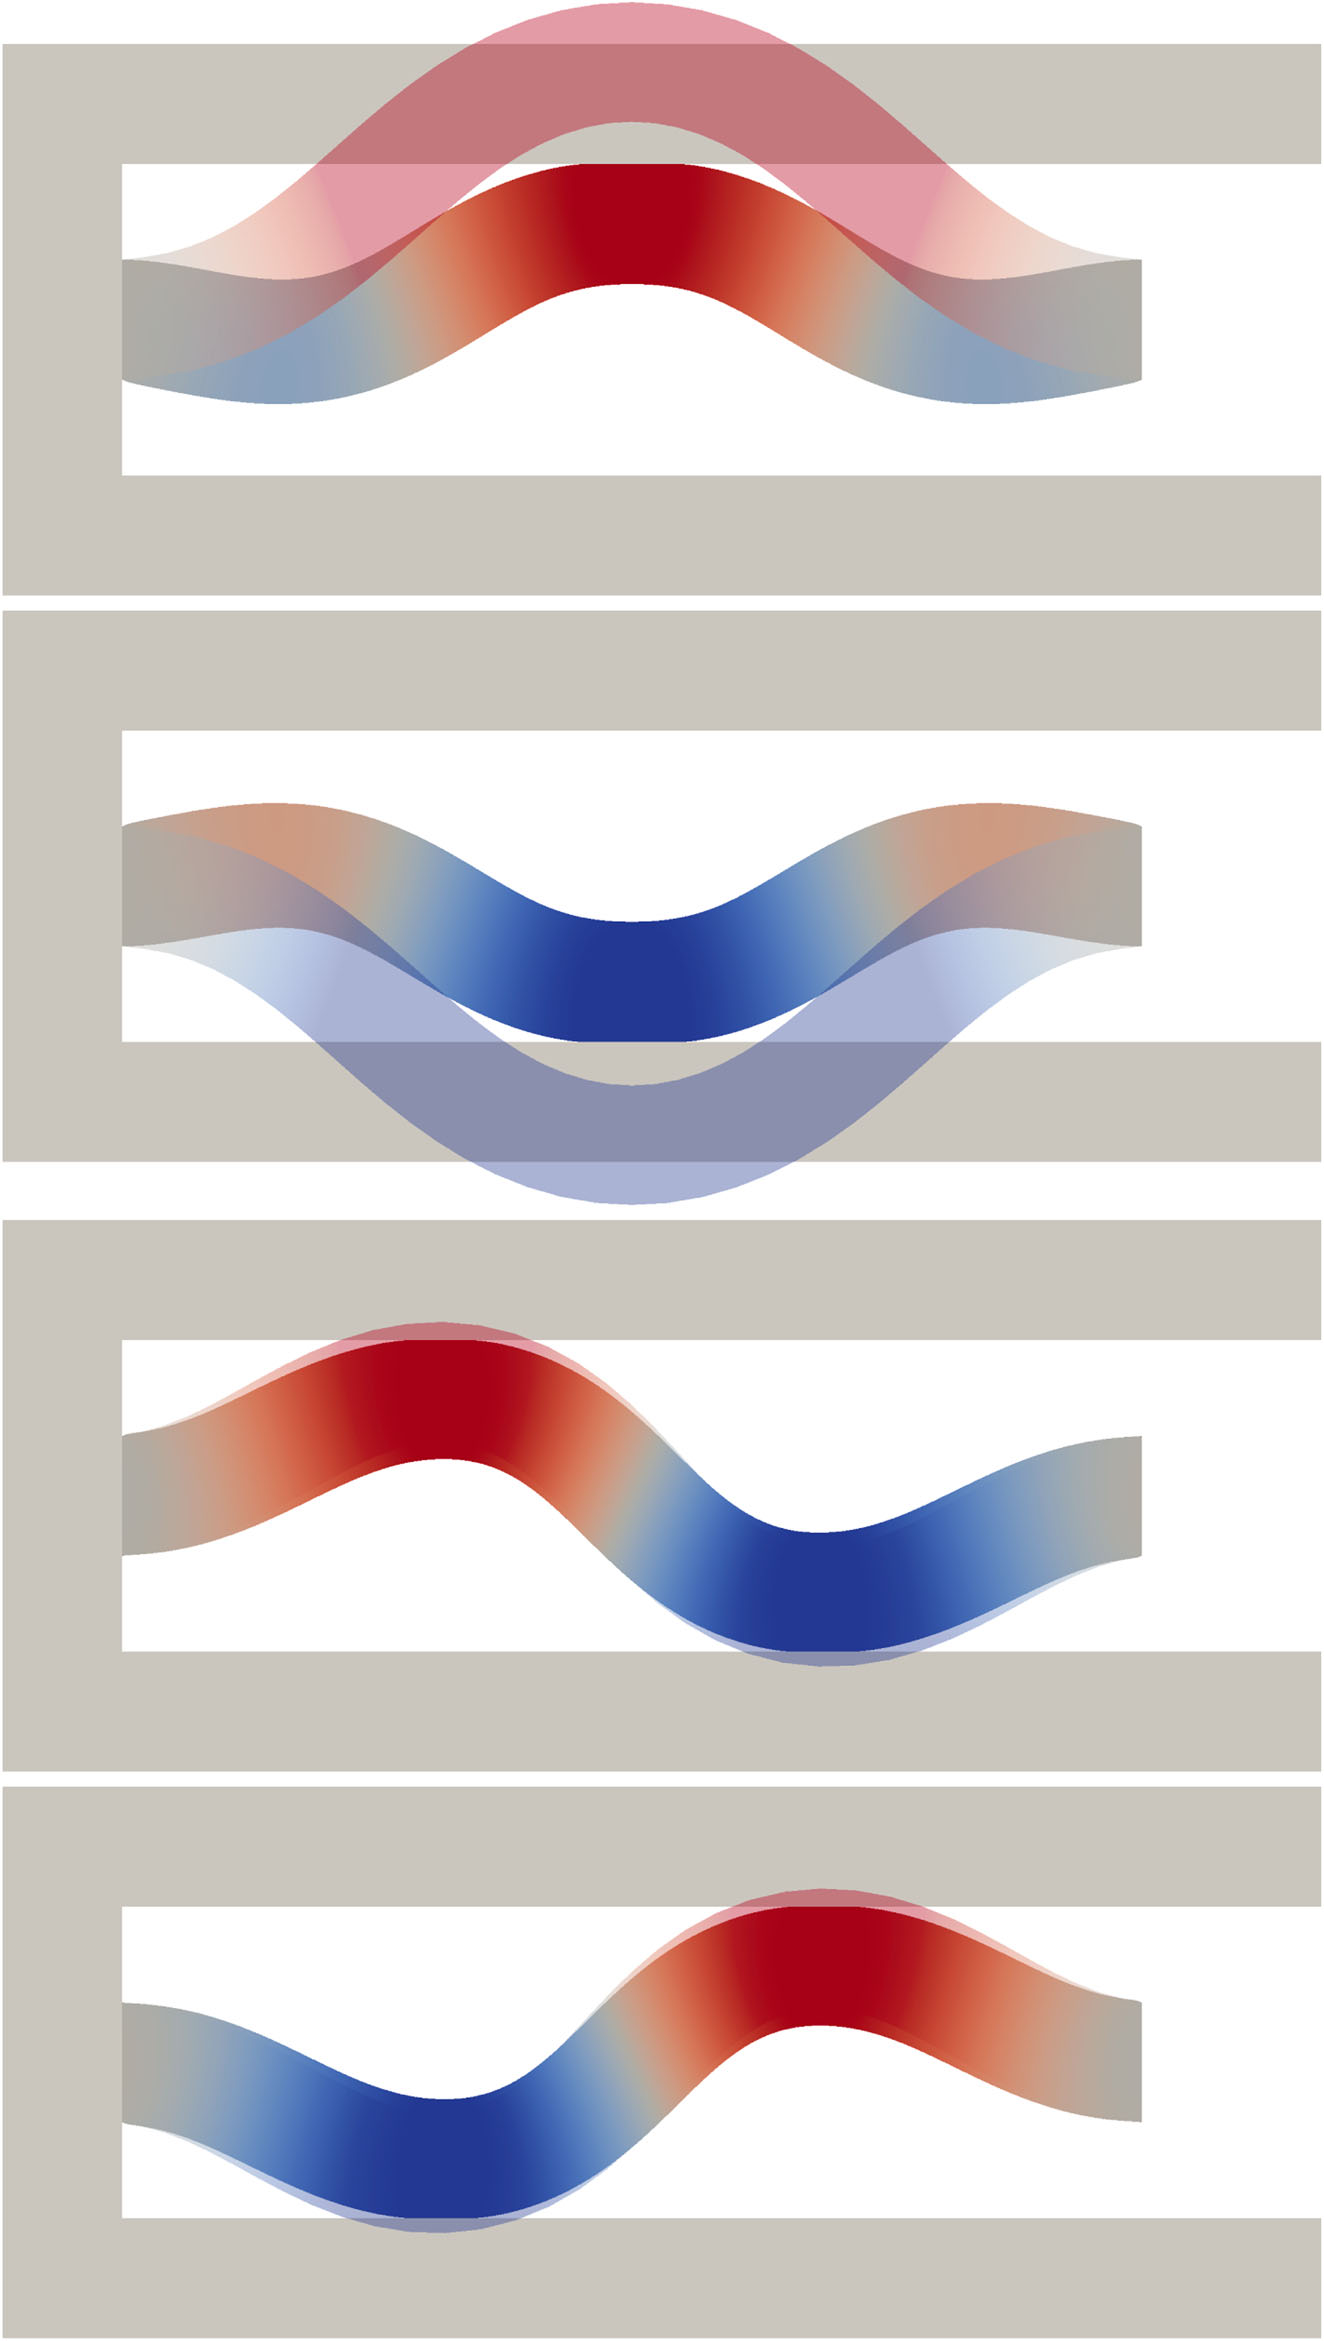
\includegraphics[height=0.8\textheight]{figs/farrell2020-fig2.jpg}
    \end{column}
  \end{columns}
\end{frame}

\begin{frame}{a fluid layer in a climate}
  a thin fluid layer moves on a substrate, with mass added (precipitation, accumulation)
  or removed (evaporation, ablation) by a signed source $f$, the \emph{climate}
  \begin{center}
    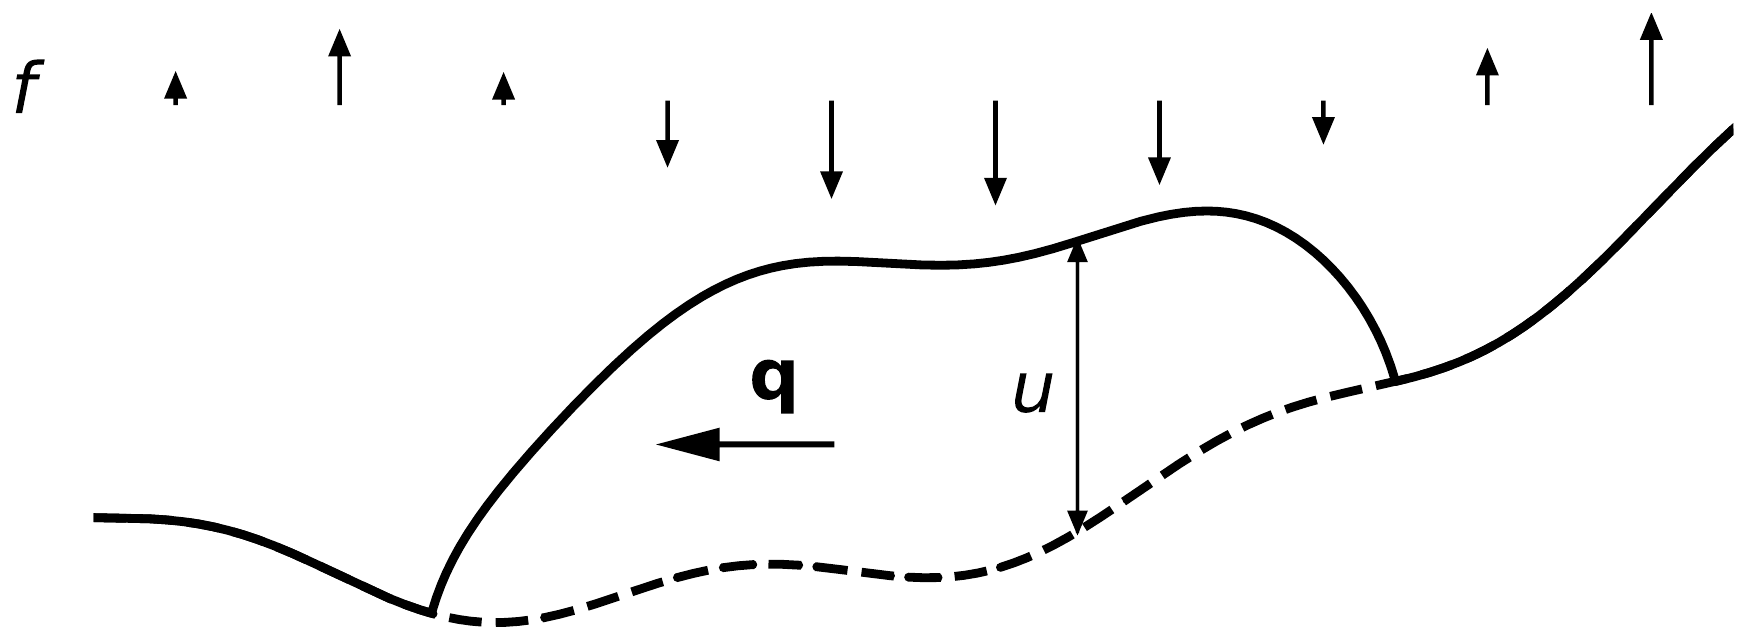
\includegraphics[width=0.45\textwidth]{figs/bueler2021-fig1.png}
  \end{center}
  thickness $u(x,t)\ge 0$, flux $q=q(\nabla u,u,x,t)$, e.g.~$q=-D\nabla u+Xu$:
  $$
    u_t+\nabla\cdot q = f \quad \text{where } u>0, \qquad\qquad u\ge 0 \quad\text{everywhere}
  $$
  \vspace{-2mm}
  \begin{itemize}
    \item glaciers and ice sheets, sea ice, subglacial water, rain on a windshield
    \item the fluid-covered area is a \alert{leading-order} modeling goal \grey{(e.g.~albedo)}
  \end{itemize}
  {\scriptsize \grey{Bueler, \emph{Conservation laws for free-boundary fluid layers}, SIAM J.~Appl.~Math.~2021}}
\end{frame}

\begin{frame}{fluid layer: one implicit time step}
  \begin{columns}[T]
    \begin{column}{0.6\textwidth}
      given $u_{n-1}\ge0$, find $u_n\ge0$ so that
      $$
        \frac{u_n-u_{n-1}}{\Delta t}+\nabla\cdot Q_n = F_n \quad \text{where } u_n>0
      $$
      this decomposes $\Omega$ into disjoint sets:
      \begin{align*}
        \Omega_n         &= \{u_n>0\} \\
        \Omega_n^r       &= \{u_n=0 \text{ and } u_{n-1}>0\} \quad \grey{\text{retreat}} \\
        \Omega_n^{00}    &= \{u_n=0 \text{ and } u_{n-1}=0\}
      \end{align*}
      \vspace{-2mm}
      \uncover<2->{
      VI on $\cK=\{v\in W^{1,p}(\Omega) : v\ge 0\}$: for all $v\in\cK$,
      $$
        \int_\Omega \frac{u_n-u_{n-1}}{\Delta t}(v-u_n) - Q_n\cdot\nabla(v-u_n)
        \ge \int_\Omega F_n\,(v-u_n)
      $$}
    \end{column}
    \begin{column}{0.38\textwidth}
      \centering
      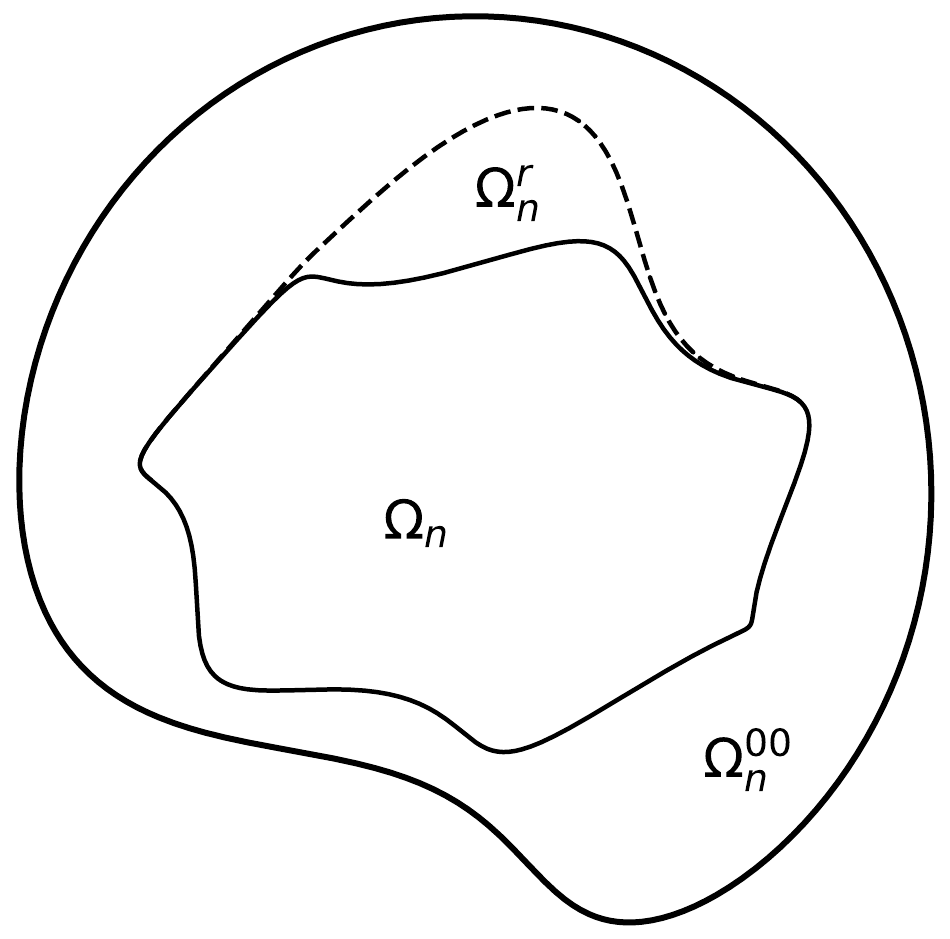
\includegraphics[width=0.85\textwidth]{figs/bueler2021-fig3.png}

      \medskip
      \raggedright
      {\small on $\Omega_n^r\cup\Omega_n^{00}$: \, $u_{n-1}+\Delta t\,F_n\le 0$}

      \smallskip
      {\small \grey{mass is \emph{not} exactly conserved on the retreat set}}
    \end{column}
  \end{columns}
\end{frame}

\begin{frame}{examples so far}
  \begin{center}
    \begin{tabular}{llll}
      \toprule
      problem                & unknown          & constraint in $\cK$     & minimization? \\
      \midrule
      obstacle               & $u\in H^1$       & $u\ge\psi$              & convex \\
      Signorini              & $u\in H^1(\Omega;\mathbb{R}^2)$ & $u\cdot n\le g$ on $\Gamma_C$ & convex \\
      hyperelastic contact   & $u\in W^{1,p}(\Omega;\mathbb{R}^2)$ & $u\cdot n\le g$ on $\Gamma_C$ & nonconvex \\
      fluid layer time step  & $u_n\in W^{1,p}$ & $u_n\ge 0$              & generally not \\
      \bottomrule
    \end{tabular}
  \end{center}
  \begin{itemize}
    \item in each, a PDE holds on an \emph{unknown} subset, and the constraint holds on the rest
    \item the VI is posed on all of $\Omega$, with no reference to the free boundary
    \item \emph{next:} when does such a VI have a unique solution?
  \end{itemize}
\end{frame}


\section[FE solutions]{finite element solutions}

\begin{frame}{foo}

  \begin{itemize}
    \item bar
  \end{itemize}
\end{frame}


\section[theory]{theory: well-posedness and an \emph{a priori} error estimate}

\begin{frame}{existence and uniqueness}
  \begin{theorem}[Stampacchia 1964]
    let $a(\cdot,\cdot)$ be bounded and coercive on a Hilbert space $V$, and
    $\cK\subset V$ nonempty, closed, convex; then for each $\ell\in V'$ there is a
    unique $u\in\cK$ with
    $$ a(u,v-u)\ge \ell(v-u) \quad\forall v\in\cK $$
  \end{theorem}
  \pause
  \begin{itemize}
    \item proof: Banach fixed point for $u\mapsto P_\cK\big(u-\rho(Au-\ell)\big)$
    \item generalizes Lax--Milgram, which is the case $\cK=V$
  \end{itemize}
\end{frame}

\begin{frame}{Falk's a priori estimate}
  for $P_1$ elements on a quasi-uniform mesh, with $\cK_h\not\subset\cK$ in general,
  $$
    \|u-u_h\|_{H^1} \le C\Big(
      \inf_{v_h\in\cK_h}\|u-v_h\| + \inf_{v\in\cK}\|u_h - v\| \Big)^{1/2}
      \lesssim C\,h
  $$
  \grey{Falk, Math.\ Comp.\ 1974}
\end{frame}


\begin{frame}{summary}

  foo
\end{frame}


\begin{frame}[standout]
  Questions?
\end{frame}


\begin{frame}{references}
  \fontsize{7}{8.2}\selectfont % inputed at end of talk1.tex

\begin{itemize}\setlength{\itemsep}{0pt}
\item E.~Bueler (2021). \emph{Conservation laws for free-boundary fluid layers}, SIAM J.~Appl.~Math.~81 (5), 2007--2032 \sdoi{10.1137/20M135217X}
\item R.~Falk (1974).  \emph{Error estimates for the approximation of a class of variational inequalities}, Math.~Comp.~28 (128), 963--971 \sdoi{10.1090/S0025-5718-1974-0391502-8}
\item P.~G.~Ciarlet (1988). \emph{Mathematical Elasticity, Vol.~I: Three-Dimensional Elasticity}, North-Holland
\item P.~Farrell, M.~Croci \& T.~Surowiec (2020). \emph{Deflation for semismooth equations}, Optim.~Methods Softw.~35 (6), 1248--1271 \sdoi{10.1080/10556788.2019.1613655}
\item G.~Fichera (1964). \emph{Problemi elastostatici con vincoli unilaterali: il problema di {S}ignorini con ambigue condizioni al contorno}, Atti Accad.~Naz.~Lincei Mem.~Cl.~Sci.~Fis.~Mat.~Natur.~Sez.~I (8) 7, 91--140
\item P.~Hartman \& G.~Stampacchia (1966). \emph{On some non-linear elliptic differential-functional equations}, Acta Math.~115, 271--310 \sdoi{10.1007/BF02392210}
\item N.~Kikuchi \& J.~T.~Oden (1988). \emph{Contact Problems in Elasticity: A Study of Variational Inequalities and Finite Element Methods}, SIAM \sdoi{10.1137/1.9781611970845}
\item D.~Kinderlehrer \& G.~Stampacchia (1980). \emph{An Introduction to Variational Inequalities and their Applications}, Academic Press; SIAM reprint 2000 \sdoi{10.1137/1.9780898719451}
\item J.-L.~Lions \& G.~Stampacchia (1967). \emph{Variational inequalities}, Comm.~Pure Appl.~Math.~20 (3), 493--519 \sdoi{10.1002/cpa.3160200302}
\item A.~Signorini (1933). \emph{Sopra alcune questioni di statica dei sistemi continui}, Ann.~Scuola Norm.~Sup.~Pisa Cl.~Sci.~(2) 2 (2), 231--251
\item G.~Stampacchia (1964). \emph{Formes bilin\'eaires coercitives sur les ensembles convexes}, C.~R.~Acad.~Sci.~Paris 258, 4413--4416
\end{itemize}

\end{frame}


\appendix

\begin{frame}{backup: projection onto a convex set}
  $P_\cK v$ is the unique $w\in\cK$ with $\ip{v-w}{z-w}\le 0$ for all $z\in\cK$
\end{frame}

\end{document}
